% =============================================================================
% SVVVL Research Paper — A No-Nonsense Walkthrough of Causal-LLM Inference
% Scaffolded from template/svvvl_paper_template.tex. Shared house-style preamble
% is preserved; the only deliberate, documented deviation is a widened right
% margin + \sidenote macro (Schwichtenberg-style margin notes) and TikZ.
% =============================================================================

\documentclass[11pt]{article}

% ----- Page geometry -------------------------------------------------------
% PAPER-SPECIFIC DEVIATION: the right margin is widened and a marginpar gutter
% is reserved so margin notes (the No-Nonsense device) have somewhere to live.
% The house default is left/right=0.85in with no marginpar column.
\usepackage[
  letterpaper,
  top=0.9in,
  bottom=0.9in,
  left=0.85in,
  right=2.05in,
  marginparwidth=1.45in,
  marginparsep=0.18in,
  headheight=14pt
]{geometry}

% ----- Encoding & language -------------------------------------------------
\usepackage[utf8]{inputenc}
\usepackage[T1]{fontenc}
\usepackage[english]{babel}



% ----- Typography ----------------------------------------------------------
\usepackage{XCharter}

% Section headings
\usepackage{titlesec}
\titleformat{\section}
  {\normalfont\Large\bfseries}{\thesection}{0.6em}{}
\titleformat{\subsection}
  {\normalfont\large\bfseries}{\thesubsection}{0.6em}{}
\titlespacing*{\section}{0pt}{1.4em}{0.6em}
\titlespacing*{\subsection}{0pt}{1.1em}{0.4em}

% Remove section numbering
\setcounter{secnumdepth}{0}

% ----- Spacing & paragraphs ------------------------------------------------
\usepackage{setspace}
\setstretch{1.15}
\setlength{\parskip}{0.6em}
\setlength{\parindent}{0pt}

% ----- Graphics & color ----------------------------------------------------
\usepackage{graphicx}
\usepackage{xcolor}
\definecolor{linkcolor}{HTML}{1F4E79}
\definecolor{svvvlblue}{HTML}{1F4E79}
\definecolor{maskgray}{HTML}{D9D9D9}
\definecolor{cellblue}{HTML}{CFE0F1}
\definecolor{cellgreen}{HTML}{D6E8D5}
\definecolor{cellgold}{HTML}{F3E4C0}

% ----- Hyperlinks ----------------------------------------------------------
\usepackage[
  colorlinks=true,
  linkcolor=linkcolor,
  urlcolor=linkcolor,
  citecolor=linkcolor
]{hyperref}

% ----- Tables, figures, captions ------------------------------------------
\usepackage{booktabs}
\usepackage{array}
\usepackage{caption}
\captionsetup{font=small, labelfont=bf, skip=6pt}

% ----- Math ----------------------------------------------------------------
\usepackage{amsmath, amssymb}
\usepackage{amsthm}
\usepackage{mathtools}

% ----- Diagrams ------------------------------------------------------------
% PAPER-SPECIFIC: TikZ for the pipeline, embedding lookup, causal attention
% matrix, transformer block, and output distribution.
\usepackage{tikz}
\usetikzlibrary{matrix, positioning, fit, arrows.meta, backgrounds, calc, shapes.geometric}

% ----- Margin notes --------------------------------------------------------
% PAPER-SPECIFIC: \sidenote{...} places a small italic aside in the right
% margin, the signature No-Nonsense device. marginnote works inside floats and
% does not consume a footnote counter, which is what we want for asides.
\usepackage{marginnote}
\renewcommand*{\marginfont}{\footnotesize\itshape\color{black!72}}
\newcommand{\sidenote}[1]{\marginnote{\setstretch{1.0}#1}}

% ----- Footnotes -----------------------------------------------------------
\usepackage[hang, flushmargin]{footmisc}
\setlength{\footnotesep}{0.8em}

% ----- Headers & footers ---------------------------------------------------
\usepackage{fancyhdr}
\pagestyle{fancy}
\fancyhf{}
\renewcommand{\headrulewidth}{0pt}
\fancyfoot[C]{\thepage}

\fancypagestyle{firstpage}{%
  \fancyhf{}%
  \renewcommand{\headrulewidth}{0pt}%
}


% ----- Logo lockup ---------------------------------------------------------
% Two levels deep (research_papers/<paper>/): reach shared assets with ../../
% and forward slashes (a backslash is parsed as a control sequence).
\newcommand{\WORDMARKFILE}{../../assets/SVVVL_Research_Wordmark.pdf}
\newcommand{\WORDMARKWIDTH}{1.5in}
\newcommand{\LOCKUPGAP}{0.01in}

% The lockup itself: symbol above wordmark, both centered within a box
% the width of the symbol so the wordmark sits naturally beneath it.
\newcommand{\logolockup}{%
  \begin{minipage}{\WORDMARKWIDTH}
    \centering
    \includegraphics[width=\WORDMARKWIDTH]{\WORDMARKFILE}
  \end{minipage}%
}

% Title block command: \makecover{Title}{Subtitle}{Authors}{Date}
\newcommand{\makecover}[4]{%
  \thispagestyle{firstpage}%
  \noindent\logolockup\par
  \vspace{2.2em}
  {\fontsize{26pt}{30pt}\selectfont\bfseries
   \hyphenpenalty=10000\exhyphenpenalty=10000\sloppy
   #1\par}
  \vspace{0.6em}
  {\fontsize{15pt}{18pt}\selectfont\itshape\color{black!70}
   \hyphenpenalty=10000\exhyphenpenalty=10000\sloppy
   #2\par}
  \vspace{1.6em}
  {\normalsize\color{black!60} #3\par}
  \vspace{0.2em}
  {\normalsize\color{black!60} #4\par}
  \vspace{1.8em}
}

% ----- Theorem environments ------------------------------------------------
\newtheorem{proposition}{Proposition}
\newtheorem{remark}{Remark}
\newtheorem{conjecture}{Conjecture}
\newtheorem{theorem}{Theorem}
\newtheorem{lemma}{Lemma}
\newtheorem{corollary}{Corollary}
\newtheorem{definition}{Definition}

% ----- Custom commands -----------------------------------------------------
% General-purpose math operators reused across papers.
\newcommand{\E}{\mathbb{E}}
\newcommand{\Var}{\mathrm{Var}}
\newcommand{\Corr}{\mathrm{Corr}}
\newcommand{\dd}{\mathrm{d}}

% Paper-specific notation for the causal-LLM walkthrough.
\newcommand{\vocab}{V}                      % vocabulary size
\newcommand{\seqlen}{T}                      % context / sequence length
\newcommand{\dmodel}{C}                      % residual-stream width (channels)
\newcommand{\nheads}{n_{h}}                  % number of attention heads
\newcommand{\dhead}{d_{h}}                   % per-head width
\newcommand{\Reals}{\mathbb{R}}
\newcommand{\softmax}{\operatorname{softmax}}
\newcommand{\LN}{\operatorname{LayerNorm}}
\newcommand{\GELU}{\operatorname{GELU}}
\newcommand{\Attn}{\operatorname{Attention}}
\newcommand{\We}{W_{E}}                      % token-embedding matrix
\newcommand{\Wp}{W_{P}}                      % positional-embedding matrix
\newcommand{\Wq}{W_{Q}}
\newcommand{\Wk}{W_{K}}
\newcommand{\Wv}{W_{V}}
\newcommand{\Wo}{W_{O}}
\newcommand{\xres}{\mathbf{x}}               % a residual-stream vector
\newcommand{\veca}[1]{\mathbf{#1}}
\newcommand{\transp}{^{\top}}

% =============================================================================
\begin{document}
% =============================================================================

% --- COVER -------------------------------------------------------------------
\makecover
  {A No-Nonsense Walkthrough of How a Causal Language Model Thinks}
  {The forward pass of a decoder-only transformer, one step at a time}
  {J.~E. Whitehead~III\footnote{SVVVL, Towson, MD, United States.
   Contact: \href{mailto:james.whitehead@svvvl.com}{james.whitehead@svvvl.com}.
   See Disclosures at the end of this document.}}
  {\today}

% --- EPIGRAPH ----------------------------------------------------------------
\vspace{-0.5em}
\begin{quote}
\itshape
``What I cannot create, I do not understand.''\\
\textnormal{--- Richard Feynman}
\end{quote}
\vspace{0.5em}

% --- ABSTRACT ----------------------------------------------------------------
\begin{quote}
\itshape
A causal language model turns a list of tokens into a guess for the next one.
That is the whole job. Everything between the input and the guess is arithmetic
you can follow by hand. This document follows it. We pick one tiny, fully
specified model --- a nano-GPT with about eighty-five thousand numbers in it,
whose only skill is sorting six letters into order --- and push a single input
through it from the first lookup to the last probability. Every arrow is named,
every matrix has a shape, and every step is the same step the giant models take,
only smaller. By the end you should be able to redraw the machine from memory.
\end{quote}


\newpage
% --- HOW TO READ THIS --------------------------------------------------------
\section{How to read this}

Most explanations of language models reach for an analogy and stop there. The
machine, we are told, ``pays attention'' or ``predicts the next word.'' True, and
useless: you cannot rebuild a thing from a verb. \sidenote{The Feynman test on the
cover is the standard we hold ourselves to. If you cannot draw the box and label
its arrows, you have not understood the box.} This walkthrough takes the opposite
stance. We will be relentlessly concrete. There is exactly one model in these
pages, it has exactly one job, and we will trace exactly one input through it.

The plan is simple. First we meet the model and its task. Then we walk the
forward pass in the order the data flows: \emph{embedding}, \emph{layer norm},
\emph{self-attention}, \emph{projection}, \emph{the MLP}, and how those snap
together into a \emph{transformer block}. We stack a few blocks, read off a
\emph{probability distribution} over the vocabulary, and \emph{decode} an actual
next token. Finally we explain the one trick --- the \emph{KV cache} --- that
makes this fast enough to be worth doing. \sidenote{This ordering is borrowed
from Bycroft's interactive visualization~[\hyperlink{ref:5}{5}], which is the
best way to \emph{see} what we here write down.}

Three habits will help. \textbf{Watch the shapes.} Every quantity is an array,
and the only way to misunderstand a transformer is to lose track of which axis is
which. We print the shape of everything. \textbf{Trust the residual stream.}
There is one central object --- a stack of $\seqlen$ vectors, each of width
$\dmodel$ --- and almost every operation reads from it and writes back to it.
Keep your eye on that stack. \textbf{Believe the smallness.} The model here is so
small you could, in principle, do its arithmetic on paper. That is the point.
GPT-3 is the same diagram with bigger numbers.

% --- THE MODEL WE WILL FOLLOW ------------------------------------------------
\section{The model we will follow}

Meet \textbf{nano-GPT}. \sidenote{This is the toy from Karpathy's
minGPT~[\hyperlink{ref:4}{4}], the same one Bycroft animates. We did not invent
it; we borrow it because it is small enough to hold in your head.} Its entire
purpose in life is to sort. You hand it a short sequence of letters drawn from
the alphabet $\{\texttt{A},\texttt{B},\texttt{C}\}$, and it emits the same letters
in sorted order. Give it \texttt{B\,C\,A\,B\,A\,C} and the right answer is
\texttt{A\,A\,B\,B\,C\,C}. That is the whole task. It is a deliberately stupid
job, chosen so that nothing about the \emph{task} distracts from the
\emph{machinery}.

A language model does not see letters. It sees \textbf{token ids} --- integers.
Our vocabulary has $\vocab = 3$ symbols, so we map
\[
  \texttt{A} \mapsto 0, \qquad \texttt{B} \mapsto 1, \qquad \texttt{C} \mapsto 2 .
\]
The model reads a context of at most $\seqlen = 6$ tokens at a time. \sidenote{$\seqlen$
is the \emph{context length}: the longest input the position machinery is built
for. Bigger models stretch this to thousands or millions; the idea is identical.}
Internally it represents each token as a vector of width $\dmodel = 48$ --- the
\emph{channels}, or the width of the \emph{residual stream}. It has $\nheads = 3$
attention heads, so each head works in a slice of width $\dhead = \dmodel/\nheads
= 16$. It stacks $L = 3$ transformer blocks. Add it all up and there are about
$85{,}000$ trainable numbers. Table~\ref{tab:scale} at the end shows how those
same dials read on GPT-2 and GPT-3; the architecture does not change, only the
sizes.

Two warnings before we start, both about what inference is \emph{not}.
\sidenote{\textbf{Inference vs.\ training.} Everything here is the forward pass
with the weights already fixed. How those $85{,}000$ numbers got their values ---
gradient descent over examples --- is a different story we do not tell.} First, we
are watching a trained model \emph{run}, not learn. Every matrix below is a fixed
table of numbers; nothing changes as data flows through. Second, the model is
\textbf{causal}: when it forms its representation of the token at position $t$, it
is allowed to look at positions $1,\dots,t$ but never at positions after $t$. That
one rule --- the past may inform the present, the future may not --- is what makes
the model a \emph{causal} (or \emph{autoregressive}) language model, and it shows
up concretely as a triangle of forbidden entries in Section~5.

\begin{figure}[t]
\centering
\resizebox{\textwidth}{!}{%
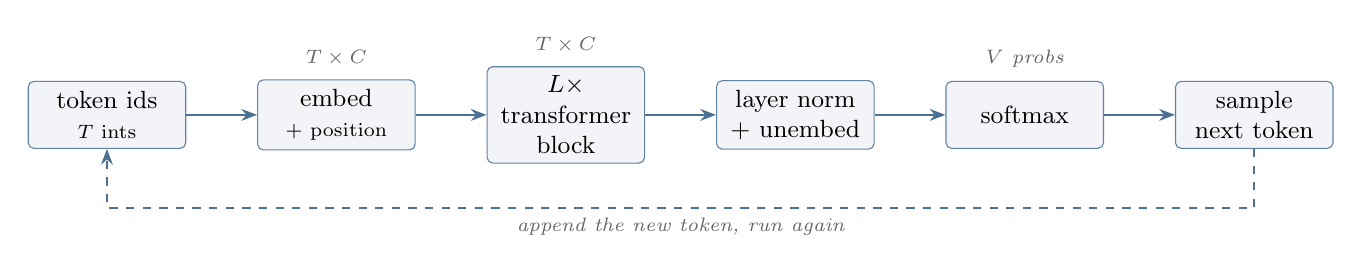
\begin{tikzpicture}[
  font=\small,
  box/.style={draw=svvvlblue!70, rounded corners=2pt, fill=svvvlblue!6,
              minimum width=2.0cm, minimum height=0.85cm, align=center},
  flow/.style={-{Stealth[length=2mm]}, svvvlblue!80, thick},
  lbl/.style={font=\scriptsize\itshape, text=black!60}
]
  \node[box] (tok)   {token ids\\\scriptsize $\seqlen$ ints};
  \node[box, right=0.9cm of tok]  (emb)  {embed\\\scriptsize $+$ position};
  \node[box, right=0.9cm of emb]  (blk)  {$L\times$\\transformer\\block};
  \node[box, right=0.9cm of blk]  (un)   {layer norm\\$+$ unembed};
  \node[box, right=0.9cm of un]   (sm)   {softmax};
  \node[box, right=0.9cm of sm]   (samp) {sample\\next token};

  \draw[flow] (tok) -- (emb);
  \draw[flow] (emb) -- (blk);
  \draw[flow] (blk) -- (un);
  \draw[flow] (un)  -- (sm);
  \draw[flow] (sm)  -- (samp);

  % feedback loop: append sampled token and re-run
  \draw[flow, dashed] (samp.south) -- ++(0,-0.75) -| node[lbl, pos=0.25, below]
        {append the new token, run again} (tok.south);

  \node[lbl, above=0.05cm of emb] {$\seqlen\times\dmodel$};
  \node[lbl, above=0.05cm of blk] {$\seqlen\times\dmodel$};
  \node[lbl, above=0.05cm of sm]  {$\vocab$ probs};
\end{tikzpicture}}
\caption{The whole machine. Token ids become vectors, flow through $L$ identical
transformer blocks while keeping their shape, get turned into a probability over
the vocabulary, and one token is drawn. The dashed arrow is autoregression: append
the new token and run the whole thing again.}
\label{fig:pipeline}
\end{figure}

Figure~\ref{fig:pipeline} is the entire document on one line. Each of the boxes
gets its own section below. Notice the shape annotations: from the embedding to
the final layer norm, the data is always a $\seqlen \times \dmodel$ block --- six
rows, forty-eight columns. The blocks reshape nothing; they only \emph{rewrite}
that block in place. \sidenote{This is why people call it the \emph{residual
stream}: a fixed-width river of $\dmodel$ numbers per position that each block
edits and passes on.}

% --- EMBEDDING ---------------------------------------------------------------
\section{Embedding: from integers to vectors}

\textbf{Intuition.} The model cannot multiply a letter. So the very first thing it
does is replace each token id with a learned vector --- a row pulled from a big
lookup table. A second table adds in \emph{where} the token sits. The sum is the
token's starting point in the residual stream.

\textbf{Mechanics.} Two matrices do this. The token-embedding matrix
$\We \in \Reals^{\vocab \times \dmodel}$ has one row per vocabulary symbol; the
positional-embedding matrix $\Wp \in \Reals^{\seqlen \times \dmodel}$ has one row
per slot in the context. \sidenote{``Embedding'' just means \emph{lookup}.
$\We[\,\texttt{id}\,]$ is row number \texttt{id}. No multiplication happens here,
only a table read. A one-hot times $\We$ is the same thing dressed up.} For a token
with id $u$ sitting at position $t$, the input vector is the row for the symbol
plus the row for the slot:
\begin{equation}
  \xres_t \;=\; \We[\,u\,] \;+\; \Wp[\,t\,] \;\in\; \Reals^{\dmodel}.
  \label{eq:embed}
\end{equation}
Stack these for all $\seqlen$ positions and you have the initial residual stream
$X \in \Reals^{\seqlen \times \dmodel}$ --- the block that will flow through every
later section.

Why add the position at all? Because attention, the next big operation, is
\emph{permutation-blind}: on its own it would treat \texttt{A\,B} and \texttt{B\,A}
as the same bag of tokens. \sidenote{This matters a lot for a \emph{sorting}
model. ``Which letters, in which slots'' is the entire input; strip the slots and
the task is impossible.} The positional rows break that symmetry, stamping each
vector with its slot so the model can tell first from last.

\textbf{nano-GPT instance.} Our input is \texttt{B\,C\,A\,B\,A\,C}, i.e.\ the ids
$(1,2,0,1,0,2)$ in the six slots. Position $0$
holds \texttt{B}, so its starting vector is $\We[1] + \Wp[0]$, a specific point in
$\Reals^{48}$. Do this for all six slots and $X$ is a $6 \times 48$ block of
numbers. Figure~\ref{fig:embed} shows the lookup for the first two slots.

\begin{figure}[t]
\centering
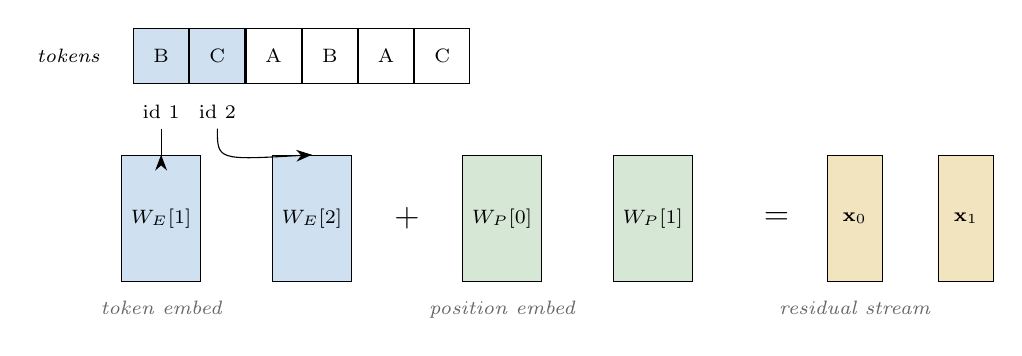
\begin{tikzpicture}[font=\small, every node/.style={font=\scriptsize}]
  % token row
  \node[draw, minimum size=0.7cm, fill=cellblue] (t0) {B};
  \node[draw, minimum size=0.7cm, right=0pt of t0, fill=cellblue] (t1) {C};
  \node[draw, minimum size=0.7cm, right=0pt of t1] (t2) {A};
  \node[draw, minimum size=0.7cm, right=0pt of t2] (t3) {B};
  \node[draw, minimum size=0.7cm, right=0pt of t3] (t4) {A};
  \node[draw, minimum size=0.7cm, right=0pt of t4] (t5) {C};
  \node[left=0.3cm of t0, font=\scriptsize\itshape] {tokens};

  % ids
  \node[below=0.15cm of t0, font=\scriptsize] (i0) {id 1};
  \node[below=0.15cm of t1, font=\scriptsize] (i1) {id 2};

  % embedding columns for first two
  \node[draw, minimum width=0.7cm, minimum height=1.6cm, below=0.9cm of t0,
        fill=cellblue] (e0) {$\We[1]$};
  \node[draw, minimum width=0.7cm, minimum height=1.6cm, right=0.9cm of e0,
        fill=cellblue] (e1) {$\We[2]$};
  \node[draw, minimum width=0.7cm, minimum height=1.6cm, right=1.4cm of e1,
        fill=cellgreen] (p0) {$\Wp[0]$};
  \node[draw, minimum width=0.7cm, minimum height=1.6cm, right=0.9cm of p0,
        fill=cellgreen] (p1) {$\Wp[1]$};

  \node[right=0.25cm of p1, font=\Large] (plus) {};

  \draw[-{Stealth[length=2mm]}] (i0.south) .. controls +(0,-0.4) .. (e0.north);
  \draw[-{Stealth[length=2mm]}] (i1.south) .. controls +(0,-0.4) .. (e1.north);

  % sum
  \node[draw, minimum width=0.7cm, minimum height=1.6cm, right=1.7cm of p1,
        fill=cellgold] (s0) {$\xres_0$};
  \node[draw, minimum width=0.7cm, minimum height=1.6cm, right=0.7cm of s0,
        fill=cellgold] (s1) {$\xres_1$};
  \node[left=0.35cm of s0, font=\large] {$=$};
  \node[font=\large] (pl) at ($(e1)!0.5!(p0)$) {$+$};

  \node[below=0.12cm of e0, font=\scriptsize\itshape, text=black!60]
        {token embed};
  \node[below=0.12cm of p0, font=\scriptsize\itshape, text=black!60]
        {position embed};
  \node[below=0.12cm of s0, font=\scriptsize\itshape, text=black!60]
        {residual stream};
\end{tikzpicture}
\caption{Embedding the first two slots of \texttt{B\,C\,A\,B\,A\,C}. The token id
selects a row of $\We$; the slot index selects a row of $\Wp$; their sum
$\xres_t = \We[u]+\Wp[t]$ is the starting vector (width $\dmodel=48$) for that
position. Repeat for all six slots to build the $6\times48$ block $X$.}
\label{fig:embed}
\end{figure}

% --- LAYER NORM --------------------------------------------------------------
\section{Layer norm: keeping the numbers civilized}

\textbf{Intuition.} As vectors pass through many layers, their entries can drift
large or small, and that wrecks the arithmetic downstream. Layer norm rinses each
vector back to a clean scale --- mean zero, unit spread --- before the expensive
operations read it. \sidenote{Think of it as resetting the volume knob before each
instrument plays, so no single channel drowns the rest.}

\textbf{Mechanics.} Layer norm acts on \emph{one vector at a time}, across its
$\dmodel$ channels. For a residual vector $\xres \in \Reals^{\dmodel}$ with entries
$x_1,\dots,x_{\dmodel}$, compute its own mean and variance,
\[
  \mu = \frac{1}{\dmodel}\sum_{i=1}^{\dmodel} x_i,
  \qquad
  \sigma^2 = \frac{1}{\dmodel}\sum_{i=1}^{\dmodel} (x_i-\mu)^2,
\]
standardize, then apply a learned per-channel scale $\gamma$ and shift $\beta$:
\begin{equation}
  \LN(\xres)_i \;=\; \gamma_i \,\frac{x_i - \mu}{\sqrt{\sigma^2 + \varepsilon}}
                 \;+\; \beta_i .
  \label{eq:ln}
\end{equation}
The tiny $\varepsilon$ just prevents a divide-by-zero. \sidenote{Crucially, the
mean and variance are computed \emph{per token, per position} --- across the
$\dmodel$ channels, not across the $\seqlen$ positions. Each of the six vectors is
normalized on its own, so the causal rule is never violated.} The vectors
$\gamma,\beta \in \Reals^{\dmodel}$ are learned, which lets the model undo the
standardization where it wants to; the normalization sets a sane baseline,
$\gamma,\beta$ keep it expressive.

\textbf{nano-GPT instance.} Each of our six $48$-vectors gets its own $\mu$ and
$\sigma$. Suppose one slot's vector has drifted to a mean of $0.7$ with a spread
of $2.3$; layer norm recenters it to mean $0$, rescales to spread $1$, then lets
the learned $\gamma,\beta$ nudge it. The shape is untouched --- in stays
$6\times48$, out stays $6\times48$. In this architecture a layer norm sits just
\emph{before} each attention and each MLP (the ``pre-norm'' arrangement), which is
why it appears twice inside every block in Section~7.

% --- SELF-ATTENTION ----------------------------------------------------------
\section{Self-attention: letting positions talk}

This is the heart of the machine, so we go slow.

\textbf{Intuition.} Up to now each position has been processed in isolation.
Attention is the one operation where positions \emph{communicate}. Every position
broadcasts a question, every position broadcasts a label, and every position
offers a payload. \sidenote{The standard names: \emph{query} = the question I am
asking, \emph{key} = the label you advertise, \emph{value} = the content you hand
over if I pick you.} A position then gathers payloads from the others in
proportion to how well its question matches their labels. For our sorting task you
can imagine a position thinking ``I need to know how many \texttt{A}s came before
me'' and pulling hardest on the positions holding \texttt{A}s.

\textbf{Mechanics, step by step.} Work inside a single head; the head sees vectors
of width $\dhead$. From each normalized residual vector we form three projections
using learned matrices $\Wq,\Wk,\Wv$:
\begin{equation}
  Q = X\Wq, \qquad K = X\Wk, \qquad V = X\Wv,
  \qquad Q,K,V \in \Reals^{\seqlen \times \dhead}.
  \label{eq:qkv}
\end{equation}
\emph{Step 1 --- scores.} Compare every query with every key by dot product. The
score of position $t$ attending to position $s$ is $Q_t \cdot K_s$. Collect them
into a $\seqlen \times \seqlen$ matrix and scale:
\begin{equation}
  S = \frac{QK\transp}{\sqrt{\dhead}} \in \Reals^{\seqlen \times \seqlen}.
  \label{eq:scores}
\end{equation}
The $\sqrt{\dhead}$ keeps the dot products from growing with width, which would
otherwise push the next step into saturation. \sidenote{Without the
$1/\sqrt{\dhead}$ scaling, large dot products make the softmax nearly one-hot too
early, and gradients (at training time) vanish. It is a small fix with a big
effect.}

\emph{Step 2 --- the causal mask.} Here is where ``causal'' becomes arithmetic. A
query at position $t$ must not see keys at positions $s > t$. So before
normalizing, set every above-diagonal score to $-\infty$:
\begin{equation}
  S'_{t,s} =
  \begin{cases}
    S_{t,s} & s \le t,\\[2pt]
    -\infty & s > t.
  \end{cases}
  \label{eq:mask}
\end{equation}
\sidenote{Why $-\infty$ and not $0$? Because the next step exponentiates. $e^{-\infty}=0$,
so a masked position gets \emph{exactly} zero weight. A masked score of $0$ would
instead leak weight $e^{0}=1$.} Figure~\ref{fig:attn} draws this triangle.

\emph{Step 3 --- softmax to weights.} Turn each row of scores into a probability
distribution over the allowed positions:
\begin{equation}
  A_{t,s} = \softmax_s(S'_{t,\cdot})
          = \frac{e^{S'_{t,s}}}{\sum_{s' \le t} e^{S'_{t,s'}}}.
  \label{eq:attnweights}
\end{equation}
Each row of $A$ now sums to $1$ and is zero above the diagonal: row $t$ says how
much position $t$ borrows from each position at or before it.

\emph{Step 4 --- gather the values.} Mix the value vectors by those weights:
\begin{equation}
  \mathrm{head}(X) = A V \in \Reals^{\seqlen \times \dhead}.
  \label{eq:headout}
\end{equation}
Position $t$'s output is a weighted average of the payloads it was allowed to see.

\textbf{Multiple heads.} The model does all of this $\nheads = 3$ times in
parallel, each head with its own $\Wq,\Wk,\Wv$ and its own slice of width $\dhead$.
\sidenote{Different heads learn different ``questions.'' One might track counts of
\texttt{A}, another the most recent letter. Splitting into heads lets the model ask
several questions at once without them interfering.} The three head outputs are
concatenated back to width $\dmodel$, ready for the projection in Section~6.

\begin{figure}[t]
\centering
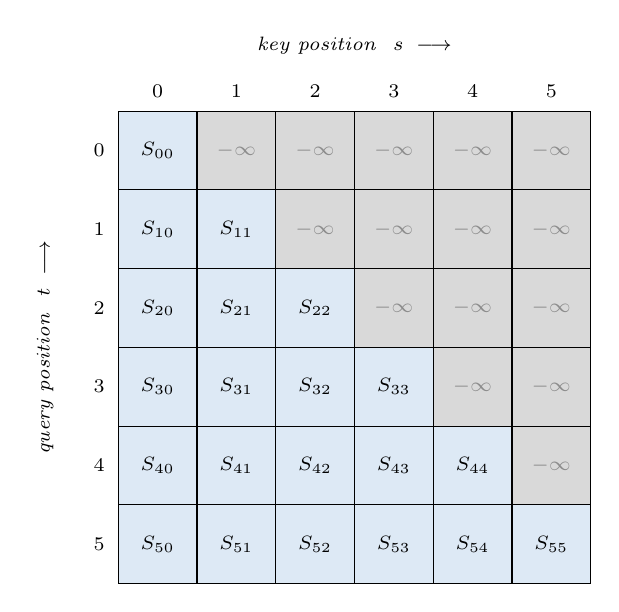
\begin{tikzpicture}[font=\scriptsize, scale=1.0]
  \def\n{6}
  \foreach \r in {0,...,5}{
    \foreach \c in {0,...,5}{
      \pgfmathtruncatemacro{\masked}{ifthenelse(\c>\r,1,0)}
      \ifnum\masked=1
        \fill[maskgray] (\c,-\r) rectangle ++(1,-1);
        \node[text=black!45] at (\c+0.5,-\r-0.5) {$-\infty$};
      \else
        \fill[cellblue!70] (\c,-\r) rectangle ++(1,-1);
        \node at (\c+0.5,-\r-0.5) {$S_{\r\c}$};
      \fi
      \draw (\c,-\r) rectangle ++(1,-1);
    }
  }
  % labels
  \foreach \c in {0,...,5}{ \node[above] at (\c+0.5,0.05) {\c}; }
  \foreach \r in {0,...,5}{ \node[left]  at (-0.05,-\r-0.5) {\r}; }
  \node[above=0.5cm] at (3,0.1) {\textit{key position } $s \;\longrightarrow$};
  \node[rotate=90, anchor=south] at (-0.7,-3)
        {\textit{query position } $t \;\longrightarrow$};
\end{tikzpicture}
\caption{The causal mask on the $6\times6$ score matrix $S$ of Eq.~\eqref{eq:scores}.
Row $t$ (a query) may attend only to columns $s \le t$ (blue); the upper triangle
($s>t$, gray) is set to $-\infty$ so that after the softmax of
Eq.~\eqref{eq:attnweights} those positions receive exactly zero weight. The future
cannot inform the past.}
\label{fig:attn}
\end{figure}

\textbf{nano-GPT instance.} With $\seqlen = 6$, each head's score matrix is
$6\times6$ and, after masking, has $1+2+3+4+5+6 = 21$ live entries out of $36$. The
first row attends only to itself; the last row may attend to all six. Each head
emits a $6\times16$ block, the three stack to $6\times48$, and we move on.

% --- PROJECTION --------------------------------------------------------------
\section{Projection: stitching the heads back together}

\textbf{Intuition.} Three heads went off and gathered information separately. The
projection mixes their findings back into a single vector per position and decides
how that mixed result should be written into the residual stream.

\textbf{Mechanics.} Concatenate the head outputs into a $\seqlen \times \dmodel$
block and multiply by the output matrix $\Wo \in \Reals^{\dmodel \times \dmodel}$:
\begin{equation}
  \mathrm{Attn}(X) = \big[\,\mathrm{head}_1 \,\|\, \cdots \,\|\, \mathrm{head}_{\nheads}\,\big]\,\Wo .
  \label{eq:proj}
\end{equation}
Then comes the move that defines the architecture --- the \textbf{residual add}.
The attention result is not the new stream; it is an \emph{edit} added onto the old
one:
\begin{equation}
  X \;\leftarrow\; X + \mathrm{Attn}(\LN(X)).
  \label{eq:resadd1}
\end{equation}
\sidenote{The residual connection is why these models train at all when stacked
deep: each block only has to learn a \emph{correction} to the stream, and the
original signal has a clear, unobstructed path forward.} Read
Eq.~\eqref{eq:resadd1} carefully: layer norm feeds attention, attention is added
back, and the un-normalized original $X$ survives on the left. The stream is never
overwritten, only nudged.

\textbf{nano-GPT instance.} The concatenated heads form a $6\times48$ block,
$\Wo$ is $48\times48$, the product is $6\times48$, and it is added onto the
$6\times48$ stream that entered the block. Shape in, shape out: $6\times48$.

% --- MLP ---------------------------------------------------------------------
\section{The MLP: thinking position by position}

\textbf{Intuition.} Attention moved information \emph{between} positions. The MLP
now processes each position \emph{on its own}, giving the model room to compute
something nonlinear with what it just gathered. \sidenote{Rough division of labor:
attention \emph{routes} information across positions; the MLP \emph{transforms} it
in place. Most of a transformer's parameters live here.}

\textbf{Mechanics.} For each position's vector, expand to a wider hidden layer,
apply a nonlinearity, and contract back. With $\GELU$ as the nonlinearity and
hidden width $4\dmodel$ (the usual choice),
\begin{equation}
  \mathrm{MLP}(\xres) = \big(\GELU(\xres W_1 + b_1)\big)\, W_2 + b_2,
  \qquad W_1 \in \Reals^{\dmodel \times 4\dmodel},\;
         W_2 \in \Reals^{4\dmodel \times \dmodel}.
  \label{eq:mlp}
\end{equation}
The same $W_1,W_2$ are applied to every position independently --- there is no
mixing across slots here, so the causal rule is automatically safe.
\sidenote{$\GELU$ is a smooth cousin of the ReLU: it lets a little negative signal
through near zero instead of hard-clipping it~[\hyperlink{ref:7}{7}].} As with
attention, the result is added back through a residual connection, after its own
layer norm:
\begin{equation}
  X \;\leftarrow\; X + \mathrm{MLP}(\LN(X)).
  \label{eq:resadd2}
\end{equation}

\textbf{nano-GPT instance.} Width in is $48$, the hidden layer is
$4\times48 = 192$, width out is $48$. Each of the six positions runs through the
same little two-layer network independently, then writes its correction back into
the stream. Shape in, shape out: $6\times48$.

% --- THE BLOCK ---------------------------------------------------------------
\section{The transformer block, assembled}

We now have all the parts. A \textbf{transformer block} is exactly the two residual
updates we just wrote, in order: normalize, attend, add; normalize, MLP, add.
\begin{align}
  X &\;\leftarrow\; X + \mathrm{Attn}\big(\LN(X)\big), \label{eq:block1}\\
  X &\;\leftarrow\; X + \mathrm{MLP}\big(\LN(X)\big). \label{eq:block2}
\end{align}
Figure~\ref{fig:block} draws it. \sidenote{Note the two layer norms sit
\emph{inside} the residual paths, before attention and before the MLP. This
``pre-norm'' layout is what almost every modern model uses; it makes deep stacks
behave.} The block takes a $\seqlen\times\dmodel$ stream and returns a
$\seqlen\times\dmodel$ stream --- same shape --- which is precisely why blocks can
be stacked without anything in between.

\begin{figure}[t]
\centering
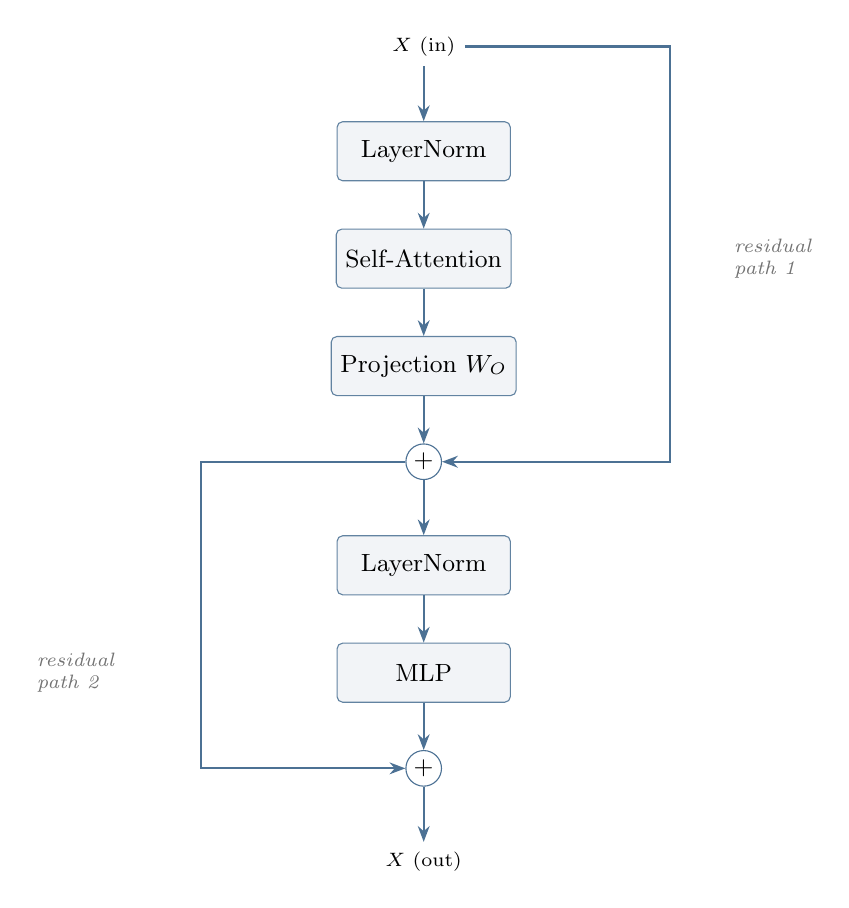
\begin{tikzpicture}[
  font=\small,
  op/.style={draw=svvvlblue!70, rounded corners=2pt, fill=svvvlblue!6,
             minimum width=2.2cm, minimum height=0.75cm, align=center},
  add/.style={draw=svvvlblue!80, circle, inner sep=1.2pt, fill=white},
  flow/.style={-{Stealth[length=2mm]}, svvvlblue!80, thick}
]
  \node (in) {\scriptsize $X$ (in)};
  \node[op, below=0.7cm of in]  (ln1)  {LayerNorm};
  \node[op, below=0.6cm of ln1] (att)  {Self-Attention};
  \node[op, below=0.6cm of att] (prj)  {Projection $\Wo$};
  \node[add, below=0.6cm of prj] (a1)  {$+$};
  \node[op, below=0.7cm of a1]  (ln2)  {LayerNorm};
  \node[op, below=0.6cm of ln2] (mlp)  {MLP};
  \node[add, below=0.6cm of mlp] (a2)  {$+$};
  \node[below=0.7cm of a2] (out) {\scriptsize $X$ (out)};

  \draw[flow] (in)  -- (ln1);
  \draw[flow] (ln1) -- (att);
  \draw[flow] (att) -- (prj);
  \draw[flow] (prj) -- (a1);
  \draw[flow] (a1)  -- (ln2);
  \draw[flow] (ln2) -- (mlp);
  \draw[flow] (mlp) -- (a2);
  \draw[flow] (a2)  -- (out);

  % residual skip 1
  \draw[flow] (in.east) -- ++(2.6,0) |- (a1.east);
  % residual skip 2
  \draw[flow] (a1.west) -- ++(-2.6,0) |- (a2.west);

  \node[right=2.7cm of att, font=\scriptsize\itshape, text=black!55, align=left]
        {residual\\path 1};
  \node[left=2.7cm of mlp, font=\scriptsize\itshape, text=black!55, align=left]
        {residual\\path 2};
\end{tikzpicture}
\caption{One transformer block, Eqs.~\eqref{eq:block1}--\eqref{eq:block2}. The
stream is normalized, passed through attention and its projection, and added back
(residual path 1); then normalized again, passed through the MLP, and added back
(residual path 2). Shape is preserved end to end, so blocks stack directly.}
\label{fig:block}
\end{figure}

\textbf{nano-GPT instance.} Our model stacks $L = 3$ of these. The $6\times48$
stream enters block~1, comes out $6\times48$, enters block~2, and so on. Three
rounds of ``route, then transform,'' each writing its small corrections into the
same river of numbers.

% --- UNEMBED + SOFTMAX -------------------------------------------------------
\section{Unembedding and softmax: from vectors to a distribution}

\textbf{Intuition.} After the last block, each position holds a rich $48$-vector.
To make a prediction we must turn the \emph{last} position's vector into a score
for every vocabulary symbol, then into probabilities. \sidenote{Why the last
position? Because in a causal model, position $t$'s output vector is the model's
summary of ``everything up to and including $t$'' --- exactly the context from
which the \emph{next} token should be predicted.}

\textbf{Mechanics.} Apply one final layer norm, then multiply by an unembedding
matrix to get \textbf{logits} --- one raw score per vocabulary symbol:
\begin{equation}
  \ell = \LN(\xres_{\seqlen})\, W_U \in \Reals^{\vocab},
  \qquad W_U \in \Reals^{\dmodel \times \vocab}.
  \label{eq:logits}
\end{equation}
Many models tie $W_U = \We\transp$ --- the same table that read tokens in is reused
to read them out. \sidenote{This ``weight tying'' saves parameters and reflects a
pleasing symmetry: the geometry that turns symbols into vectors is reused to turn
vectors back into symbols.} The logits are then squashed into a probability
distribution by the softmax:
\begin{equation}
  p_k = \softmax(\ell)_k = \frac{e^{\ell_k}}{\sum_{j=1}^{\vocab} e^{\ell_j}},
  \qquad \sum_k p_k = 1.
  \label{eq:outsoftmax}
\end{equation}

\textbf{nano-GPT instance.} The last position's $48$-vector hits $W_U$
($48\times3$) and produces three logits, one each for \texttt{A},\texttt{B},
\texttt{C}. Softmax turns them into three probabilities. For our input
\texttt{B\,C\,A\,B\,A\,C}, a well-trained model puts almost all the mass on
\texttt{A} for the first output slot, because \texttt{A} is the smallest letter and
must come first. Figure~\ref{fig:dist} sketches that distribution.

\begin{figure}[t]
\centering
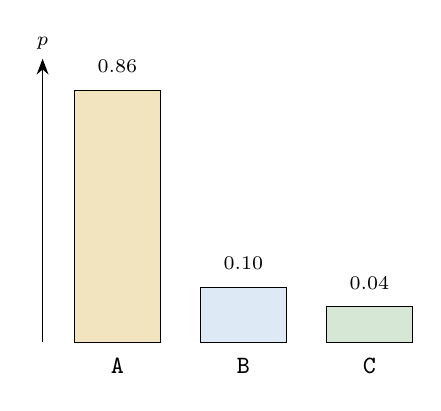
\begin{tikzpicture}[font=\small]
  \def\bw{1.1}
  % bars: A high, B medium-low, C low
  \fill[cellgold]  (0,0) rectangle (\bw,3.2);
  \fill[cellblue!70] (1.6,0) rectangle (1.6+\bw,0.7);
  \fill[cellgreen] (3.2,0) rectangle (3.2+\bw,0.45);
  \draw (0,0) rectangle (\bw,3.2);
  \draw (1.6,0) rectangle (1.6+\bw,0.7);
  \draw (3.2,0) rectangle (3.2+\bw,0.45);
  \node at (0.55,-0.3) {\texttt{A}};
  \node at (2.15,-0.3) {\texttt{B}};
  \node at (3.75,-0.3) {\texttt{C}};
  \node at (0.55,3.5) {\scriptsize $0.86$};
  \node at (2.15,1.0) {\scriptsize $0.10$};
  \node at (3.75,0.75) {\scriptsize $0.04$};
  \draw[-{Stealth[length=2mm]}] (-0.4,0) -- (-0.4,3.6) node[above,font=\scriptsize] {$p$};
\end{tikzpicture}
\caption{The output distribution from Eq.~\eqref{eq:outsoftmax} for the first
predicted slot of \texttt{B\,C\,A\,B\,A\,C}. The model concentrates probability on
\texttt{A}, the correct smallest letter. The numbers are illustrative.}
\label{fig:dist}
\end{figure}

% --- DECODING ----------------------------------------------------------------
\section{Output: turning a distribution into a token}

\textbf{Intuition.} A distribution is not yet an answer. \emph{Decoding} is the
rule that picks one concrete token from the probabilities --- and the same logits
can yield different behavior depending on the rule. \sidenote{This is the one place
the model's output is genuinely a \emph{choice}. Everything before
Eq.~\eqref{eq:outsoftmax} is deterministic arithmetic; sampling is where
randomness, if any, enters.}

\textbf{The common rules.}
\begin{itemize}\setlength{\itemsep}{0.3em}
  \item \textbf{Greedy.} Take the most probable token, $\arg\max_k p_k$.
        Deterministic; for our sorting model, the right rule --- there is one
        correct next letter.
  \item \textbf{Temperature.} Before the softmax, divide logits by a temperature
        $\tau$: $p_k \propto e^{\ell_k/\tau}$. \sidenote{$\tau<1$ sharpens the
        distribution toward greedy; $\tau>1$ flattens it toward uniform; $\tau\to0$
        \emph{is} greedy.} Low $\tau$ is conservative, high $\tau$ is adventurous.
  \item \textbf{Top-$k$ / top-$p$.} Keep only the $k$ most probable tokens (or the
        smallest set whose mass exceeds $p$), renormalize, and sample from those.
        Cuts off the long tail of bad tokens while keeping some variety.
\end{itemize}

\textbf{The autoregressive loop.} Whatever the rule, the chosen token is
\emph{appended} to the input, and the entire forward pass runs again to predict the
\emph{next} token --- the dashed arrow in Figure~\ref{fig:pipeline}. This is the
sense in which the model is autoregressive: its own output becomes its next input.

\textbf{nano-GPT instance.} Greedy decoding on Figure~\ref{fig:dist} emits
\texttt{A}. We append it, rerun, and the model --- now conditioned on the input
plus its own \texttt{A} --- emits the second sorted letter, and so on until the six
sorted letters \texttt{A\,A\,B\,B\,C\,C} are complete.

% --- KV CACHE ----------------------------------------------------------------
\section{The KV cache: why you do not redo all the work}

There is a glaring waste in the loop just described. To predict token $t+1$ we rerun
the whole forward pass on tokens $1,\dots,t$. But at the previous step we already
ran it on $1,\dots,t-1$. Almost everything is being recomputed.

\textbf{The fix.} Look back at attention. For a \emph{new} query at position $t$,
the scores it needs are $Q_t \cdot K_s$ and the payloads $V_s$ for all $s \le t$.
The keys and values $K_s, V_s$ for the \emph{old} positions $s < t$ do not depend
on the new token at all --- they were already computed. \sidenote{This works
\emph{because} the model is causal: old positions never attend to the new one, so
adding a token cannot change any past $K$ or $V$. Causality is what makes the cache
correct.} So we keep them. The \textbf{KV cache} stores the key and value vectors
of every position seen so far. At each new step the model computes $K,V$ for only
the \emph{one} new token, appends them to the cache, and attends against the whole
cache.

\textbf{What changes.} Without the cache, generating $n$ tokens costs work growing
like $n^2$ in the sequence length --- you reprocess the whole prefix every step.
With it, each step does work proportional to the current length, and the per-step
cost of re-embedding and re-running the prefix disappears. \sidenote{The cost moves
from compute to memory: the cache itself grows with the sequence length and the
number of layers, and for long contexts it, not the arithmetic, becomes the
bottleneck.} The arithmetic of any single step is exactly what we wrote in
Sections~3--9; the cache only avoids \emph{repeating} the steps for tokens whose
representations are already settled.

% --- PUTTING IT TOGETHER -----------------------------------------------------
\section{Putting it together}

Trace the whole machine once more, end to end, on \texttt{B\,C\,A\,B\,A\,C}. Six
letters become six ids; each id selects a row of $\We$ and adds a row of $\Wp$,
giving a $6\times48$ residual stream (Eq.~\eqref{eq:embed}). That stream flows
through three transformer blocks; in each, a layer norm feeds self-attention, whose
causal mask lets every position pool information only from its past
(Figure~\ref{fig:attn}), the heads are stitched by a projection and added back, and
then a per-position MLP refines each vector and is added back too
(Figure~\ref{fig:block}). After the third block, the last position's vector is
normalized, multiplied by the unembedding to three logits, and softmaxed into a
distribution over \texttt{A},\texttt{B},\texttt{C} (Eq.~\eqref{eq:outsoftmax}).
Greedy decoding reads off \texttt{A}; we append it and run again. Six passes later
the model has written \texttt{A\,A\,B\,B\,C\,C}.

Every one of those operations was small enough to check by hand. Now read
Table~\ref{tab:scale}: the same operations, the same diagram, run inside GPT-2 and
GPT-3. Nothing in the wiring changes between the toy and the giant --- only
$\dmodel$, the head count, the layer count, and the context length grow. That is
the one idea worth keeping: \emph{a frontier language model is this walkthrough,
scaled.}

\begin{table}[ht]
\centering
\caption{The same dials, three sizes. The architecture in
Figures~\ref{fig:pipeline}--\ref{fig:block} is identical across all three; only the
numbers grow. Figures are the standard published configurations.}
\label{tab:scale}
\renewcommand{\arraystretch}{1.3}
\begin{tabular}{l r r r r}
\toprule
\textbf{Quantity} & \textbf{nano-GPT} & \textbf{GPT-2 (small)} & \textbf{GPT-2 (XL)} & \textbf{GPT-3} \\
\midrule
Vocabulary $\vocab$            & 3      & 50{,}257 & 50{,}257 & 50{,}257 \\
Context length $\seqlen$       & 6      & 1{,}024  & 1{,}024  & 2{,}048  \\
Channels $\dmodel$             & 48     & 768      & 1{,}600  & 12{,}288 \\
Heads $\nheads$                & 3      & 12       & 25       & 96       \\
Blocks $L$                     & 3      & 12       & 48       & 96       \\
Parameters                     & ${\sim}85\text{k}$ & 124\,M & 1.5\,B & 175\,B \\
\bottomrule
\end{tabular}
\end{table}

\newpage
% --- REFERENCES --------------------------------------------------------------
% Hand-numbered list. Cite in text with [\hyperlink{ref:N}{N}]; each entry sets a
% matching \hypertarget{ref:N}{}. Keep numbering in sync with the list.
\section{Further Reading and References}

\begin{itemize}\setlength{\itemsep}{0.4em}

  \item[{[1]}]\hypertarget{ref:1}{} Vaswani, A., Shazeer, N., Parmar, N., Uszkoreit,
    J., Jones, L., Gomez, A.~N., Kaiser, \L., \& Polosukhin, I. (2017).
    ``Attention Is All You Need.'' \textit{Advances in Neural Information
    Processing Systems}, 30.

  \item[{[2]}]\hypertarget{ref:2}{} Radford, A., Wu, J., Child, R., Luan, D.,
    Amodei, D., \& Sutskever, I. (2019). ``Language Models Are Unsupervised
    Multitask Learners.'' \textit{OpenAI Technical Report} (GPT-2).

  \item[{[3]}]\hypertarget{ref:3}{} Brown, T.~B., Mann, B., Ryder, N., et al.
    (2020). ``Language Models Are Few-Shot Learners.'' \textit{Advances in Neural
    Information Processing Systems}, 33 (GPT-3).

  \item[{[4]}]\hypertarget{ref:4}{} Karpathy, A. (2020--2023). \textit{minGPT} and
    \textit{nanoGPT}: minimal PyTorch re-implementations of GPT.
    \texttt{https://github.com/karpathy/minGPT}.

  \item[{[5]}]\hypertarget{ref:5}{} Bycroft, B. (2023). \textit{LLM Visualization}
    --- an interactive 3D walkthrough of a GPT-style model.
    \texttt{https://bbycroft.net/llm}.

  \item[{[6]}]\hypertarget{ref:6}{} Ba, J.~L., Kiros, J.~R., \& Hinton, G.~E.
    (2016). ``Layer Normalization.'' \textit{arXiv:1607.06450}.

  \item[{[7]}]\hypertarget{ref:7}{} Hendrycks, D., \& Gimpel, K. (2016).
    ``Gaussian Error Linear Units (GELUs).'' \textit{arXiv:1606.08415}.

\end{itemize}

\newpage
% --- DISCLOSURES -------------------------------------------------------------
\section{Disclosures}

The views expressed in this document are those of the author and
SVVVL alone and do not constitute investment, legal, tax, or
accounting advice. This document is provided for informational and
research purposes only and is not an offer or solicitation to buy or
sell any security or financial product.

The framework presented is theoretical and relies on idealized
assumptions that do not hold in practice. The results
should not be implemented in a real portfolio without additional
constraints and considerations not addressed in this paper.

While reasonable care has been taken in the preparation of this
document, no representation or warranty, express or implied, is made
as to its accuracy or completeness.

Reading this document does not create an advisory, fiduciary, or
client relationship of any kind between the reader and SVVVL or the
author.

\end{document}
